\chapter{Modèle de graphe de cycles}
\label{chap3}


Dans ce chapitre, nous allons définir formellement le modèle de graphes de cycles. Le graphe de cycles d'une molécule représente la partie structurelle de  celle-ci et est construit en utilisant son graphe moléculaire. Nous construisons ce modèle pour calculer la similarité structurelle entre molécules. Ainsi, il est primordial que des molécules structurellement similaires aient des graphes de cycles similaires. 

Cette représentation de la partie structurelle d'une molécule se fait à une échelle gros-grain. On ne se situe pas à l'échelle atomique comme dans les graphes moléculaires mais à l'échelle cyclique. L'élaboration de ce modèle gros-grain appelé par la suite graphe de cycles passe d'une part par la construction d'un ensemble de cycles pertinent pour décrire la structure moléculaire et d'autre part par l'interconnexion de ces cycles en fonction de leurs interactions dans la molécule. On souhaite garantir la notion de canonicité et la proximité sur les graphes de cycles.  La canonicité signifie que deux graphes moléculaires isomorphes et ayant une numérotation de sommets différente aient des graphes de cycles isomorphes. Elle garantie également qu'à un graphe moléculaire, on associe un unique graphe de cycles quelque soit la numérotation des sommets. La proximité quand à elle signifie que si deux graphes moléculaires sont proches (elles diffèrent d'un cycle par exemple) alors les graphes de cycles le seront aussi. De plus, pour le chimiste, certains "grands" cycles dans les molécules ne définissent pas la structure de celle-ci. Il s'avère donc nécessaire de ne pas sauvegarder une certaine taille de cycles dans les graphes de cycles.

Dans la section \ref{intuition}, nous présentons et analysons une construction intuitive du graphe de cycles d'une molécule. Ensuite, nous définissons dans la section \ref{interconnexion}, le graphe de cycles qui capture la structure de cycles et l'interconnexion de ces cycles. Plus particulièrement, nous expliquons comment relier les cycles dans le graphe de cycles en respectant la structure du graphe moléculaire. Finalement dans la Section \ref{generateurcycles} nous présenterons cette section l'algorithme permettant d'avoir une base de cycles pertinente et suffisante pour capturer la partie structurelle des molécules. Nous verrons la notion d'hiérarchie pour limiter la taille des cycles dans le graphe de cycles.

\section{Une représentation intuitive du graphe de cycles }
\label{intuition}

%Lorsqu'on parle du graphe cycles modélisant l'interconnexion des cycles dans une molécule, l'un des modèles que l'on peut construire intuitivement est tel que:  l'ensemble des sommets contient des cycles pertinents qui definissent de la structure de la molécule et 

On veut construire un graphe de cycles d'une molécule basé sur sa partie structurelle. Bien que le graphe moléculaire modélise globalement l'ensemble de l'information structurelle, il n'encode pas explicitement l'information cyclique. L'hypothèse étant que des molécules similaires sont structurellement similaires et que la partie structurelle d'une molécule est défini par l'interconnexion des cycles pertinants présentes dans celle-ci. 
Un \textit{cycle pertinent} est un cycle simple et élémentaire ne pouvant être obtenu par combinaison de cycles plus petits \cite{vismara}. 

Pour s'assurer que l'on capture les cycles pertinents, on pourrait au premier abord, prendre tous les cycles de la molécule. Cependant, compter tous les cycles dans un graphe est NP-complet sachant qu'il peut y avoir un nombre exponentiel. Pour son usage dans la mesure de similarité, la représentation du graphe de cycles  d'une molécule doit contenir un nombre minimal de cycles mais suffisant pour décrire au mieux sa structure ; il s'avère donc inutile de prendre tous les cycles de la molécule pour construire le graphe de cycles.

Une base de cycles d'un graphe quand elle contient un ensembe fini de cycles élémentaires (cf. chap2). Les cycles d'une base sont pertinents. Pour construire le graphe de cycles (Figure \ref{grapheintuitif}) d'une molécule $\mathcal{M}$, nous prenons intuitivement un hypergraphe $GC = (VC,EC,\mu)$ (défini par \cite{benoit}) :
\begin{itemize}
\item L'ensemble de sommets $VC$ est une base de cycles $ \mathcal{B}$. Chaque sommet $c$ correspond à un cycle pertinent et $\mu(c)$ correspond au sous-graphe moléculaire dans $\mathcal(M)$ contenant les atomes et liasons qui appartient au cycle $c$.
\item Deux cycles $c_1$ et $c_2$  de $VC$ sont reliés par une arête si et seulement si elles partagent au moins un atome dans le graphe moléculaire de $\mathcal{M}$ c'est à dire $\mu(c_1) \cap \mu(c_2) = \emptyset$. 
\end{itemize}  

\begin{figure}[H]
\label{grapheintuitif}

\begin{center}
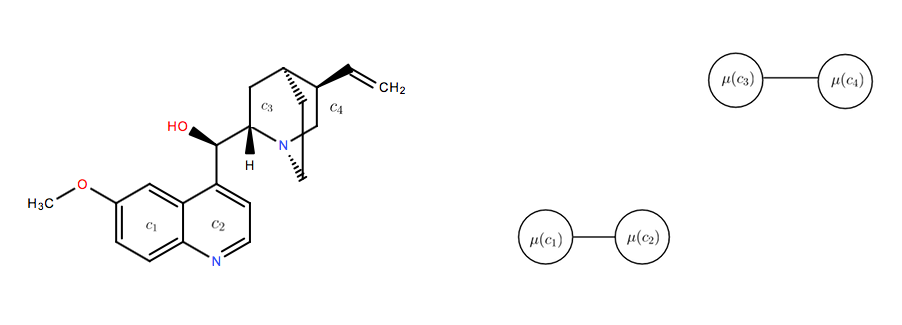
\includegraphics[scale=0.45]{exemple_intuitif_correct.png}
\end{center}
\caption{Graphe moléculaire de la quinine et le graphe de cycles intuitif associé}
\end{figure}

En observant le graphe de cycles de la Figure \ref{grapheintuitif}, on ne peut pas savoir exactement si le graphe moléculaire possède $2$ composantes connexes ou dans le contraire, sur quel cycle entre $c_1$ et $c_2$ les cycles $c_3$ et $c_4$ sont liées dans $\mathcal{M}$. Es-ce le cycle $c_3$ qui est relié au cycle $c_1$ ? ou au cycle $c_2$ ? ou à la fois à $c_1$ et $c_2$?

On pourrait tout à fait donner comme graphes moléculaires associés au graphe de cycles de la quinine, les graphes de la Figure \ref{exempleintuitif}.

\begin{figure}[H]
\label{exempleintuitif}

\begin{center}
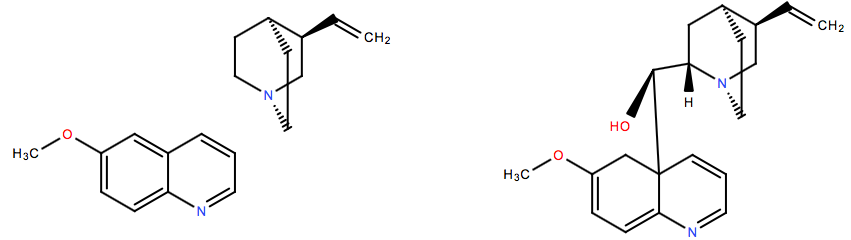
\includegraphics[scale=0.45]{exemple_graphes.png}
\end{center}
\caption{Graphes moléculaires ayant le même graphe de cycles que la quinine.}
\end{figure}

On constate dès lors que ce modèle n'est pas suffisant notamment :
\begin{itemize}
\item Au niveau de l'interconnexion des cycles: il semble logique que deux cycles ayant des atomes en commun soient liés dans $GC$ mais il faudrait aussi rajouter des liens supplementaires entre cycles indirectement liés pour réduire l'ambigüité et mieux décrire la structure des molécules.

\item Au niveau de la base de cycles : Elle n'est pas nécessairement unique ! Ce qui entrainerait dans la construction du graphe de cycles que l'on puisse avoir un graphe de cycles différent en fonction de la base choisi. En terme de similarité, cela reviendrait à dire qu'une molécule n'est pas totalement similaire à elle-même.
\end{itemize} 

\section{Interconnexion des cycles}
\label{interconnexion}
Nous avons vu dans la section précédente que le graphe de cycles devrait avoir suffisamment d'arêtes pour décrire la partie structurelle de la molécule. Dans cette section nous allons définir les types d'intersections que nous utiliserons danns le graphe de cycles.


\begin{definition}
Étant donné un graphe moléculaire $\graphe{G}$ d'une molécule $\mathcal{M}$, son graphe de cycles $GC$ est défini par un graphe simple, non orienté et etiqueté  ~{$\graphecycle{G}$} tel que :

\begin{itemize}
\item L'ensemble de sommets $VC$ est constitué d'un nombre fini de cycles pertinents décrivant la structure de $\mathcal{M}$,
\item  La fonction $\phi : VC \mapsto \mathbf{N}$ pour étiqueter les sommets de $GC$,

\item L'ensemble d'arêtes $EC$ modélise les différentes interconnexions entre les sommets du graphe de cycles,
\item Les fonctions $\varphi: EC \mapsto \{1,2\}$  et $\chi: EC \mapsto \mathbf{N}$ permettent respectivement de distinguer les types d'arêtes et leurs étiquettes.

\end{itemize}
\end{definition}

Nous distinguons $2$ principaux types d'interconnexions entre cycles : les cycles directement liés et les cycles indirectement liés.

\subsection{Le type 1 : Cycles directement liés}

Deux cycles sont directement liés s'ils ont une relation directe dans la molécule. C'est à dire qu'ils partagent au moins un atome dans le graphe moléculaire de $\mathcal{M}$. Chimiquement cela signifie qu'une interaction sur l'un des cycles affecte rapidement l'autre. Si deux cycles sont reliés par une arête de ce type alors ils appartiennent à une même composante $2-$connexe. 

Soit un graphe de cycles $GC$ et deux cycles $c_1, c_2 \in VC$. Les fonctions d'étiquettages des arêtes sont telles que:

\begin{itemize}
\item $\varphi([c_1,c_2]) = 1 $ si l'arête est de type $1$,
\item $\chi([c_1,c_2]) $ pour une arête de type $1$ est égale au nombre de liaisons chimiques en commun entre les cycles $c_1$ et $c_2$.
\end{itemize} 

Si $c_1$ et $c_2$ partagent un seul atome alors  $\chi([c_1,c_2]) = 0$.

\begin{exemple} Le cycle élémentaire $c_2$ (situé au milieu du graphe moléculaire) est lié de part et d'autre par des arêtes de type $1$. On constate aussi que le cycle $c_1$ et $c_3$ ne sont pas liés. Cette connexion n'est pas nécessaire car le graphe de cycle fournit l'information du voisin commun $c_2$ entre les cycles $c_1$ et $c_3$.

\begin{figure}[H]
\label{type1}

\begin{center}
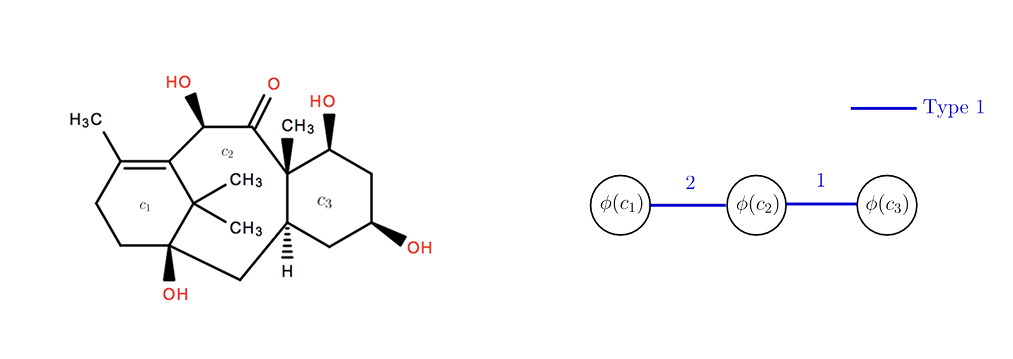
\includegraphics[scale=0.85]{type1_exemple.png}
\end{center}
\caption{Graphe moléculaire et graphe de cycles }
\end{figure}

\end{exemple}

\subsection{Le type 2 : Cycles indirectement liés}

Deux cycles sont indirectement liés lorsqu'ils sont reliés dans le graphe moléculaire par des chaînes. Dans la Figure \ref{grapheintuitif}, on a constaté qu'il fallait des informations supplémentaires pour décrire en la partie strcutrelle de la molécule.


Bien que les cycles $c_2$ et $c_3$ de la Figure \ref{type2} ne partagent pas d'atomes, une arête entre ces deux cycles dans $GC$ permettrait de lever l'ambiguïté.

Soit un graphe de cycles $GC$ et deux cycles $c_1, c_2 \in VC$. Les fonctions d'étiquettages des arêtes sont telles que:

\begin{itemize}
\item $\varphi([c_1,c_2]) = 2 $ si l'arête est de type $2$. C'est à dire qu'il existe dans $G$ une chaîne d'atomes ne passant par aucun cycle de $VC$ reliant les cycles $c_1$ et $c_2$,
\item $\chi([c_1,c_2]) $ pour une arête de type $2$ est égale à la longueur de la plus petite chaîne reliant $c_1$ et $c_2$ dans $G$.
\end{itemize} 

\begin{exemple} Les cycles élémentaires $c_2$ et $c_3$ appartiennent à deux composantes $2-$connexes différentes. La plus petite chaîne relaint ces $é$ cycles est de longueur $2$.

\begin{figure}[H]
\label{type2}

\begin{center}
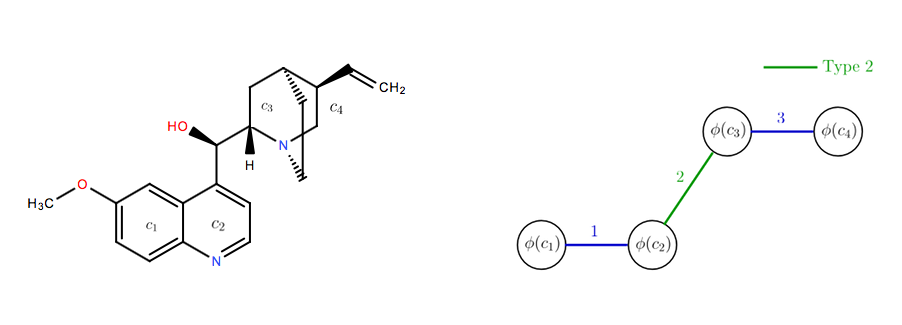
\includegraphics[scale=0.45]{type2_exemple.png}
\end{center}
\caption{Graphe moléculaire et graphe de cycles }
\end{figure}

\end{exemple}

Maintenant que nous avons défini les types d'interconnexions, nous allons procédér au choix de la base de cycles pour construire le graphe de cycles.

\section{ Le générateur pour le graphe de cycles}
\label{generateurcycles}


On rappelle que l'on souhaite avoir une représentation canonique de la partie structurelle de la molécule. Dans cette section, nous allons construire l'ensemble de sommets $VC$ et définir la fonction $\phi(VC)$. 

\subsection{Une base de cycles comme générateur ?}


Une base de cycles de longueur minimum est un candidat potentiel pour construire le graphe de cycles. Il contient un nombre fini de cycles et toutes les bases de cycles d'un graphe ont le même nombre de cycles.

En reprenant le graphe moléculaire de la quinine, on constate dans la Figure \ref{lesbases} que ce graphe possède $3$ bases de cycles différentes. Deux cycles de l'ensemble $\{c_3, c_4, c_5\}$ suffisent pour obtenir une base.

\begin{figure}[H]
\label{lesbases}

\begin{center}
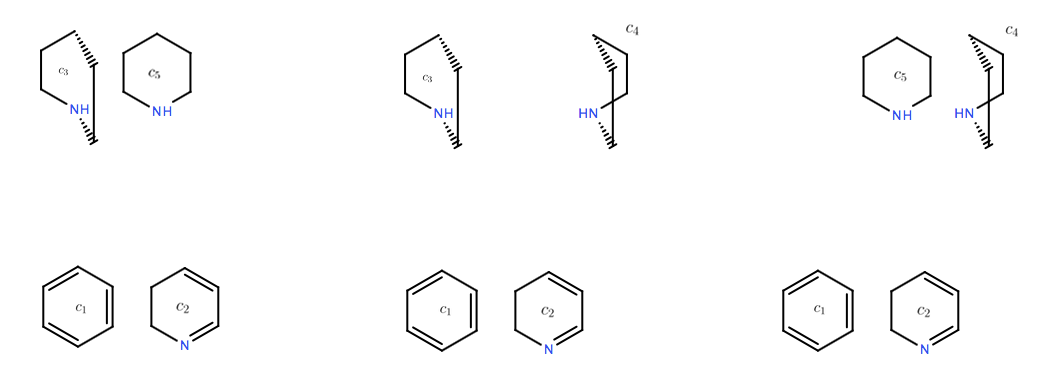
\includegraphics[scale=0.75]{base_complete.png}
\end{center}
\caption{Les bases de cycles pour le graphe moléculaire de la quinine}
\end{figure}

En construisant les graphes de cycles avec chacune de ces bases on obtient respectivement $GC_1$,$GC_2$ et $GC_3$. Les graphes $GC_2$ et $GC_3$ sont isomorphes. Le choix d'une base de cycle pourrait donner un graphe de cycles différent pour une même molécule.


\begin{figure}[H]
\label{bases}

\begin{center}
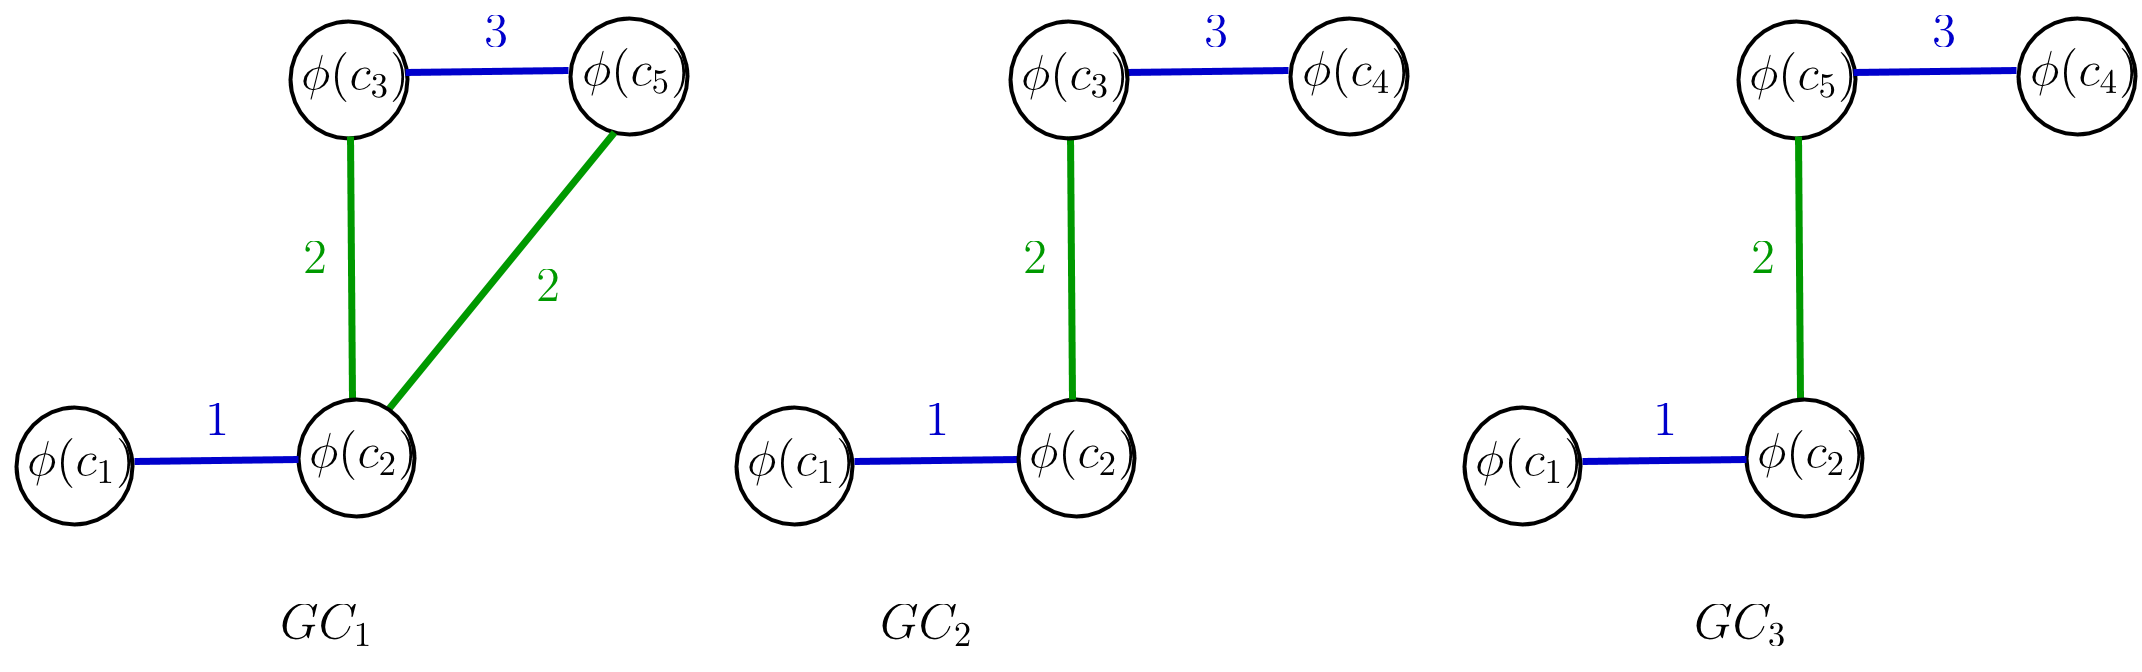
\includegraphics[scale=0.35]{graphes_base.png}
\end{center}

\caption{Les graphes de cycles pour les différentes bases de cycles.}
\end{figure}
Dans ce cas, si on prend deux fois la même molécule et deux bases de cycles différentes, la mesure de similarité concluerait que les graphes de cycles ne sont pas totalement similaires. 


Cela deviendrait encore plus ambigüe s'il existe des cycles raccrochés au composé xxxx (voir Figure \ref{differentsgraphes}). Si on continue d'étendre ce graphe moléculaire, les graphes de cycles d'une molécule pourraient prêter à confusion pour la similarité. 

\begin{figure}[H]
\label{differentsgraphes}
\begin{center}
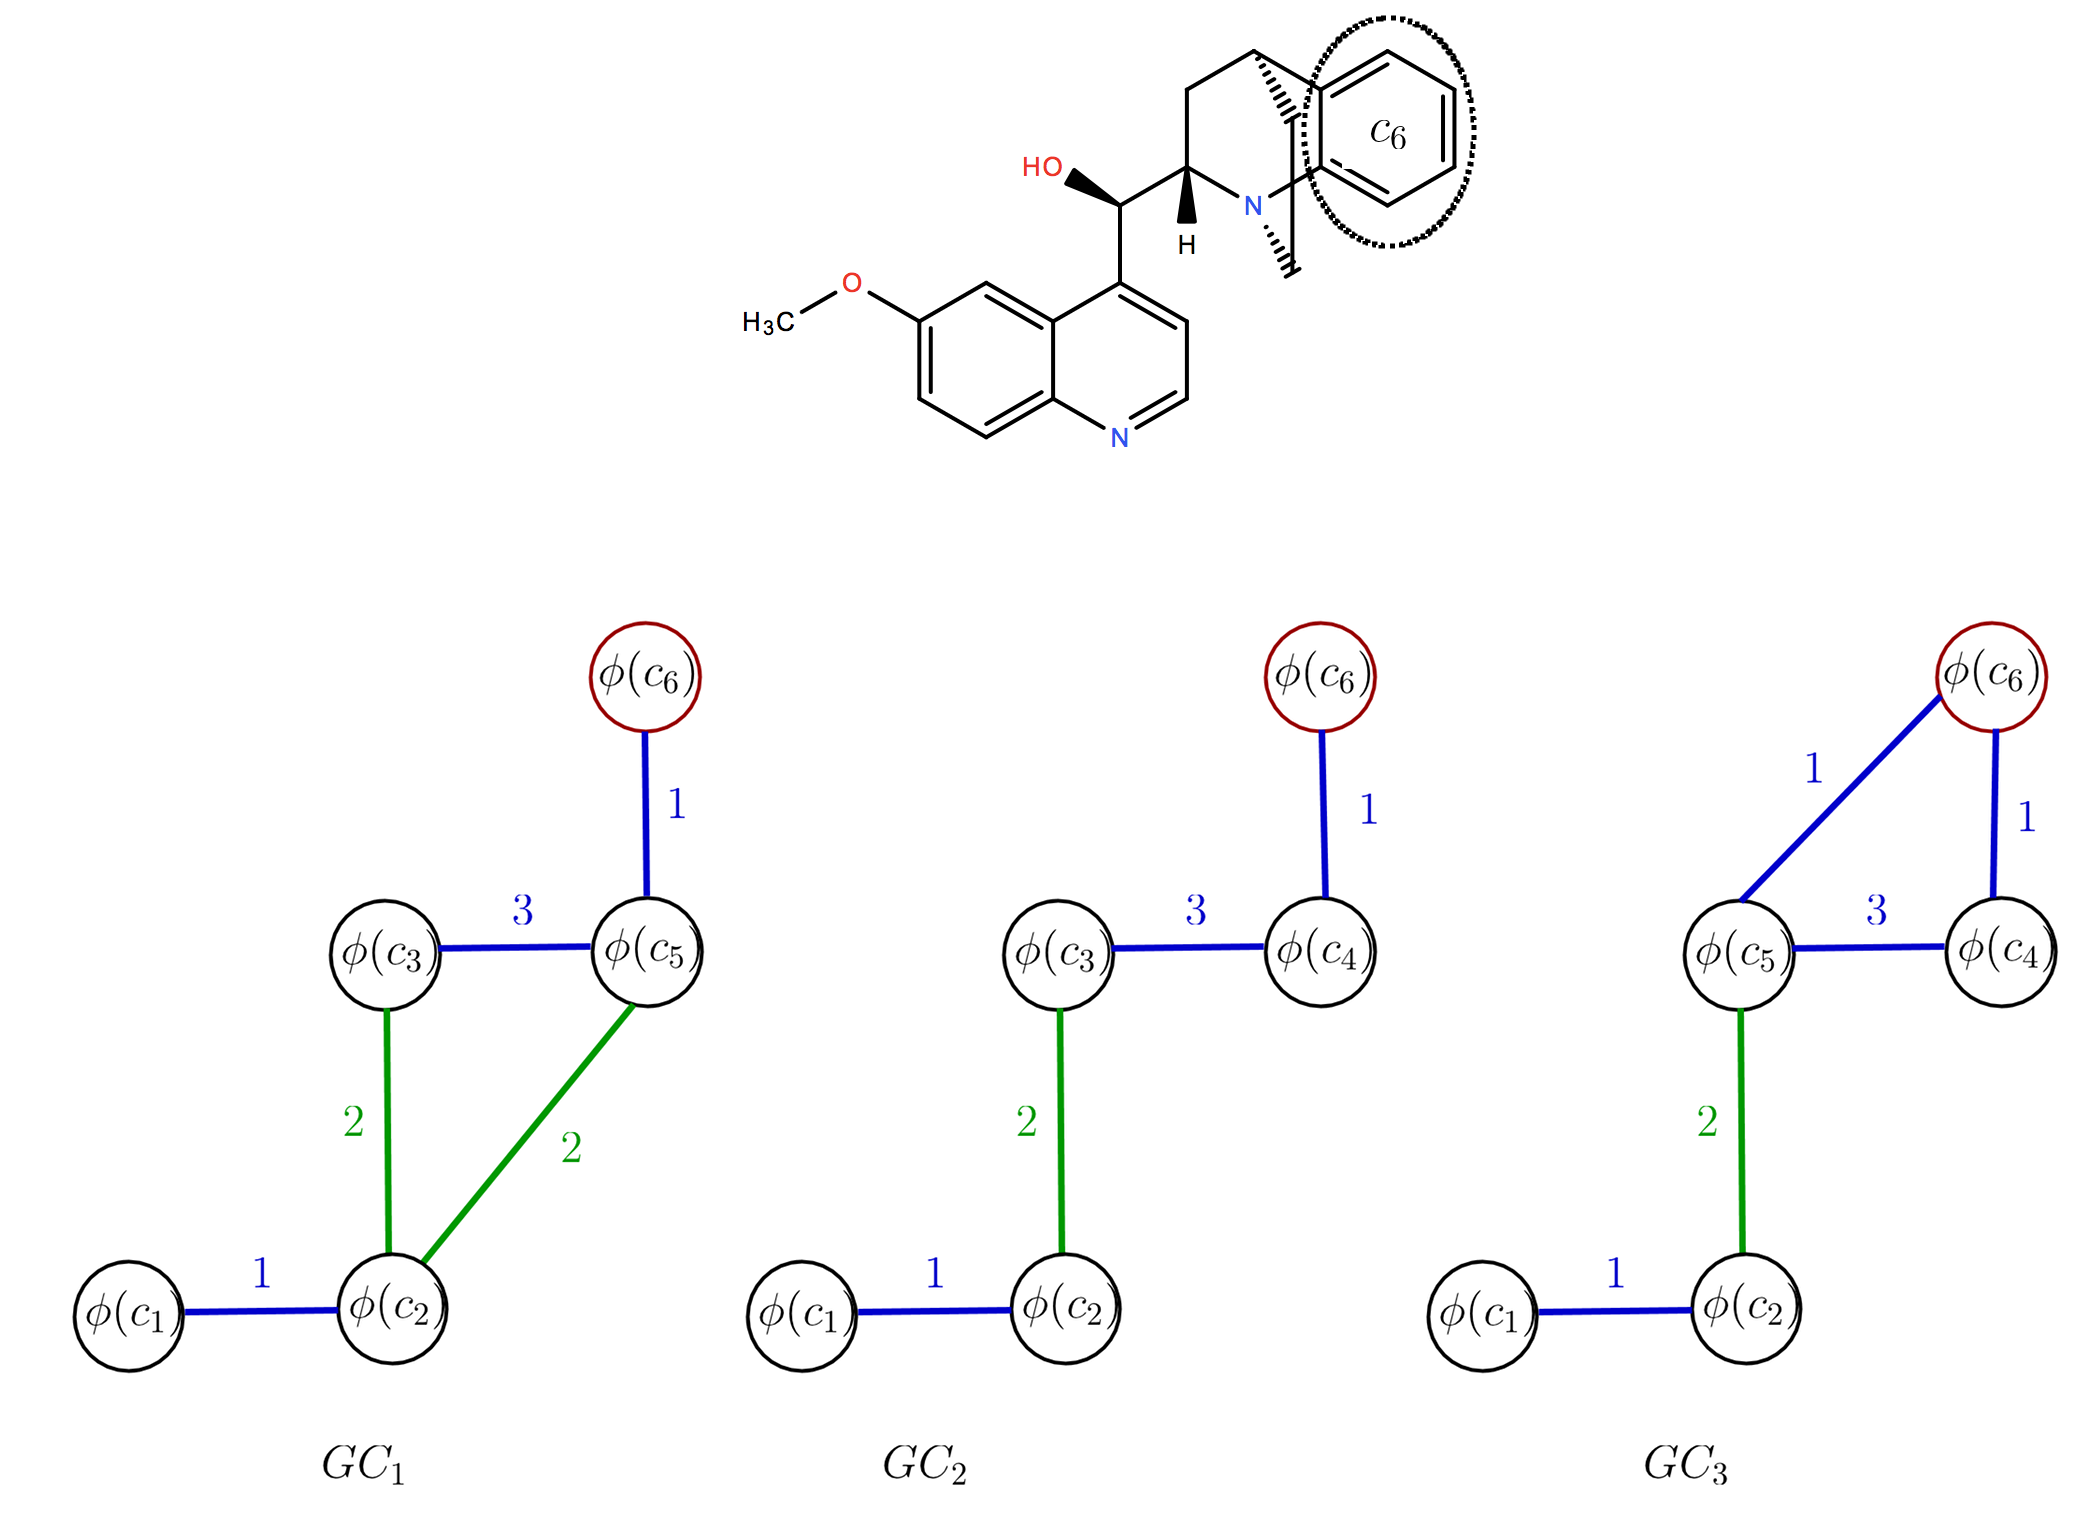
\includegraphics[scale=0.4]{graphes_different.png}
\end{center}
\caption{L'ajout d'un cycle dans un graphe moléculaire augmente potentiellemnt le nombre de graphes de cycles possibles.}
\end{figure}

En observant l'algorithme de Horton, précisement au niveau de la selection des cycles indépendants, deux des cycles $c_3, c_4$ et $c_5$ seront selectionnés en fonction de l'ordre de classement qui n'est pas prédefini.


%\subsection{Générateur canonique}

Pour construire un générateur canonique pour le graphe de cycles, nous utilisons l'algorithme de Horton et l'algorithme de McKay.  La première étape consiste à numéroter canoniquement les sommets du graphe moléculaire en utilisant l'algorithme d'isomorphisme de McKay. Ensuite, cette numérotation de sommets est utilisée pour obtenir une base de cycle de longueur minimum $\mathcal{B}$ avec l'algorithme de Horton. Et finalement, on rajoute eventuellement des cycles pour garantir la canonicité.

\subsection{Algorithme de McKay pour la numérotation canonique}

Cet algorithme a été conçu pour résoudre le problème d'isomorphisme de graphes. Décider de l'existence d’un isomorphisme entre deux graphes $G_1$ et $G_2$ est dans NP. L'algorithme de Brendan McKay \cite{Hartke} cherche un étiquetage canonique des sommets d'un graphe permettant leur ordonnancement. Si deux graphes possèdent le même étiquetage alors ils sont isomorphes \cite{McKay201494}. 

Cependant le problème peut être résolu en temps polynomial pour certaines classes de graphes, par exemple les graphes planaires ou les graphes de degré borné et en temps quasi-polynomial pour le cas général. Les graphes moléculaires se retrouvent dans cette catégorie car le degré des sommets est borné par le nombre de liaisons covalentes des atomes.

\begin{definition}
Une partition d'un ensemble $E$ est une collection d'ensembles disjoints deux à deux et non vides (appelées blocs dans la suite) dont l'union est $E$. Une partition ordonnée de $E$ est une partition dont on a ordonné les blocs. Lorsque chaque bloc d'une partition est de taille $1$, la partition est dite discrète. 
\end{definition}

L'algorithme de McKay commence par établir un partitionnement ordoné et équitable des sommets en fonction du degré. Une partition dans lequel les sommets du même bloc sont deux à deux adjacents à un nombre identique de sommets dans un autre bloc est une partition \textbf{équitable}. Avec une partition équitable, l'algorithme introduit des distinctions supplementaires entre les sommets. A chaque étape, il examine tous les choix pertinents en explorant systématiquement l’espace des partitions ordonnées équitables à l’aide d’un arbre de recherche. L'algorithme s'arrête lorsque chaque partition est discrète. 


Ensuite à chaque noeud final de l'arbre est une partition ordonée et discrète.  Chacune de ces partitions définit une nouvelle numérotation des sommets de $V$. La numeérotation se fait dans l'ordre dans lequel les sommets apparaisssent. %l'algorithme associe une permutation d'indices dans le graphe c'est à dire une nouvelle numérotation.

Chaque isomorphisme peut-être vu comme un mot en concatenant les ensembles de la partition.
\textcolor{red}{La numerotation canonique est l'isomorphisme ayant le mot le plus petit.pas tout a fait ! c'est un mot binaire, j'ecrirais la version exacte plus tard... DOIS JE RAJOUTER UN PETIT EXEMPLE POUR MONTRER COMMENT CA FONCTIONNNE ? } 

Cet algorithme est implémenté dans le package \textit{nauty}\cite{McKay201494} disponible sous differents systèmes d'exploitations (Windows, Mac OS, GNU/Linux).


\subsection{Algorithme de Horton pour une base de cycles}

Cet algorithme calcule une base de cycles de longueur minimum dans un graphe. Soit un graphe $G = (V,E)$, l'algorithme de Horton\cite{horton} est polynomial en $\mathcal{O} (|E|^3\times |V|)$.


Il se base sur le théorème suivant : 

\begin{theorem}
Soit un sommet $v$ appartenant à un cycle $c$ dans une base de cycles de longueur minimum $\mathcal{B}$. Alors il existe une arête $(x,y)$ dans $c$ tel que : $c = P(v,x) + P(v,y) + (x,y)$ avec $P(v,x)$ un plus court chemin entre $v$ et $x$ dans $G$.
\end{theorem}

La première étape de l'algorithme consiste à trouver s'il existe, un plus court chemin entre chaque paire de sommet. Ensuite, on verifie s'il existe des cycles élémentaires entre chaque sommet et chaque arête du graphe. Cela permet d'obtenir au maximum $|E| \times |V|$ cycles élémentaires. À l'étape $3$, les cycles sont classés par taille croissante de manière à les selectionner dans cet ordre durant la dernière étape.

\vspace{0.5cm}
\begin{algorithm}[H]
\SetAlgoLined
\KwData{Un graphe simple $G=(V,E)$}
 \KwResult{Une base de cycles de longueur minimum $\mathcal{B}$}
Trouver un plus court chemin entre chaque paire de sommets de $V$ \;
Pour chaque sommet $v$ et chaque arête $(x,y)$ du graphe $G$, créer un cycle $c(v,x,y) = P(v,x) + P(v,y) + (x,y)$\;
Ordonner les cycles par taille croissant\;
Utiliser un algorithme glouton pour extraire une base de cycles de longueur minimum à partir des cycles obtenus\;
\caption{Algorithme de Horton}
\end{algorithm} 

\vspace{0.5cm}

L'étape $4$ consiste former une matrice binaire dans laquelle chaque ligne est un cycle (en respectant l'ordre effectué à l'étape $3$). Chaque colonne représente une arête du graphe. Si une arête appartient à un cycle la case associé aura la valeur $1$ et la valeur $0
$ sinon. L'élimination de Gauss peut alors être appliquée pour obtenir une base de cycle de longueur minimum.

\textcolor{red}{Un exemple?}


\subsection{Générateur canonique}

Pour obtenir le générateur canonique $\zeta$ d'un graphe moléculaire, on calcule une base de cycles de longueur minimum $\mathcal{B}$ en ayant au préalable effectué une numérotation canonique des sommets.
Ensuite pour résoudre le prolème engendré par la chiralité, on rajoute éventuellement à $\mathcal{B}$ l'intégralité des cycles respectant la règle suivante :

\begin{center}
$\forall c,c' \in \mathcal{B}$ on calcule $c" = c \oplus c'$ en combinant $c$ et $c'$. Si $c"$ est un cycle élementaire de taille plus petite ou égale à ceux de $c$ et $c'$ alors il pertinent pour le graphe de cycles.
\end{center}

La fonction d'etiquettage des sommets $\phi$ associe à chaque cycle, sa taille c'est dire le nombre d'atomes qu'il contient dans le graphe moléculaire.

Dans la figure \ref{graphequinine}, le graphe de cycles de la quinine conserve alors les trois cycles du composé chiral. Ces cycles partagent alors des arêtes de type $1$ avec $\phi(c_i)$ , la taille du cycle $c_i$.

\begin{figure}[H]
\label{graphequinine}
\begin{center}
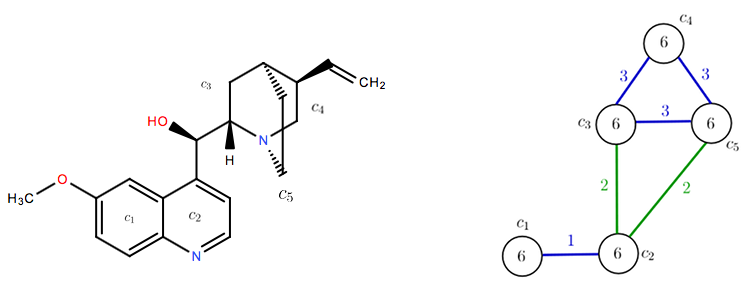
\includegraphics[scale=0.45]{graphe_quinine.png}
\end{center}
\caption{Le graphe de cycles $GC$ de la quinine.}
\end{figure}

La complexité de l'algorithme qui calcule le graphe de cycles d'un graphe $G$ est $\mathcal{O}(n^2.m^3)$.


\subsection{Générateur j-hierarchique }

Nous allons introduire la notion de $j-$hierarchique avec l'exemple suivant:

\begin{exemple}
On considère deux molécules struturellement similaires : la Strychnine et la Vomicine. Sur la figure \ref{hierarchiqueexemple}, si on prend en compte tous les cycles du générateur canonique, alors on trouverait que les graphes de cycles associés à ces molécules ne sont pas assez similaires avec en mesurant la similarité. 

\begin{figure}[H]
\label{hierarchiqueexemple}
\begin{center}
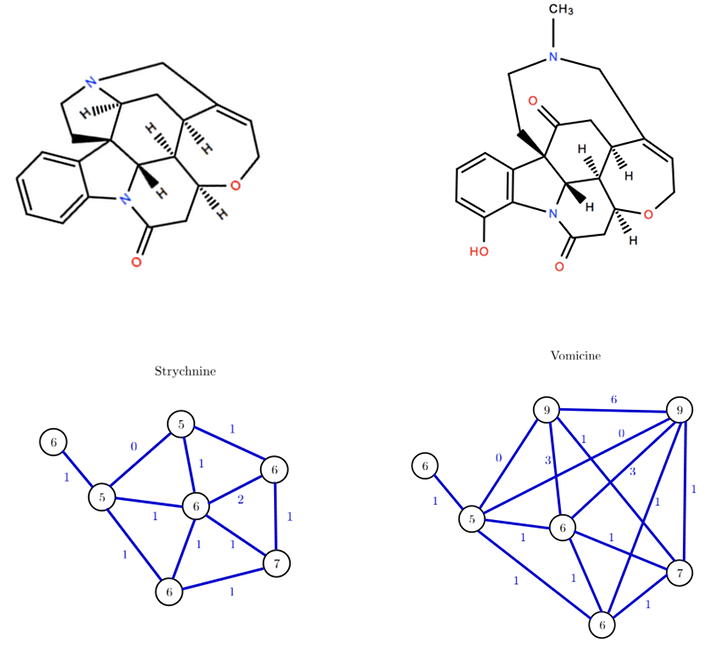
\includegraphics[scale=0.85]{j-hierarchique.png}
\end{center}
\caption{Les molécules : Strychnine et Vomicine avec leur graphe de cycles.}
\end{figure}
En effet, deux cycles de la Strychnine (de taille respectivent $5$ et $6$) ont fusionnés entraînant l'apparition de deux cycles de taille $9$ dans le graphe de cycles de la Vomicine. De plus, ces cycles ne sont pas chimiquement pertinents pour la Vomicine.

Si on reprend le générateur canonique de la Vomicine et on supprime les cycles de taille $9$, le nouveau graphe de cycles obtenu (dans la figure \ref{newjhierarchique}) capte mieux sa similarité avec la Strychnine.

\begin{figure}[H]
\label{newjhierarchique}
\begin{center}
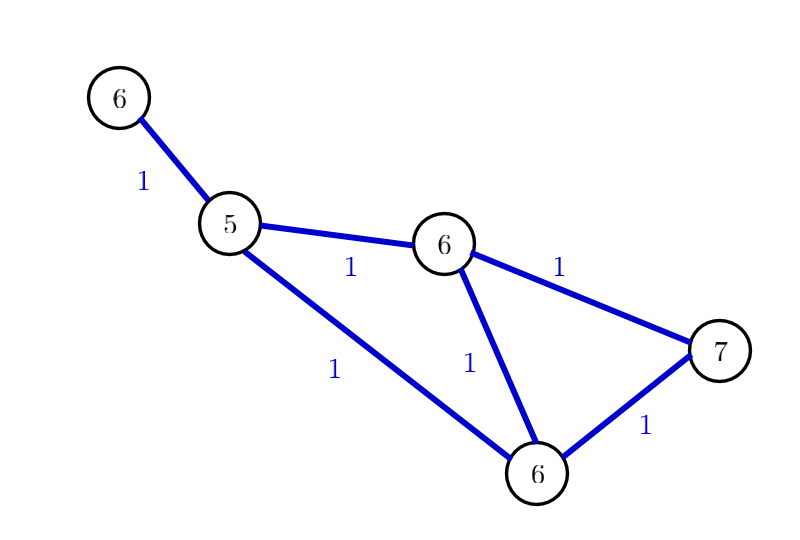
\includegraphics[scale=0.5]{gc_vomicine.png}
\end{center}
\caption{Le graphe de cycles de la Vomicine en supprimant les cycles de taille $9$.}
\end{figure}

%En effet, un cycle pertinent dans la Strychnine a été cassé pour obtenir la Vomicine. Cette modification de la structure de la Strychnine donne lieu à d'autres cycles plus grands et non pertinent pour la structure de la Vomicine.
\end{exemple}


\begin{definition}
Soit un générateur canonique $\zeta$ et un entier $j$. Le générateur $\zeta$ est $j-$hierarchique si le sous-ensemble contenant tous les cycles de $\zeta$ ayant une taille inférieure ou égale à $j$ génère tous les cycles de $G$ ayant une taille inférieure ou égale à $j$.
\end{definition}

Un générateur est \textit{hierarchique} si et seulement si il est $j-$hierarchique pour tout $j$. On note $\zeta_j$ le générateur $j-$hierarchique de $\zeta$. Le générateur canonique utilisé pour construire le graphe de cycles est hierarchique car la base de cycles de longueur minimum l'es.


\begin{lemme}
Toute base de cycles de longueur minimum d'un graphe est hierarchique.
\end{lemme}

\begin{preuve}
Soit $G$ un graphe et $\mathcal{B}$ une base de cycles de longueur minimum de $G$. $\forall j, \mathcal{B}_j$ est une base de cycles de longueur minimum pour les cycles de longueur inférieur ou égal $j$.

Supposons que $\mathcal{B}$ n'est pas hierarchique; Cela signifie qu'il existe un entier $j$ tel que $\mathcal{B}_j$ n'est pas $j-$hierarchique.

Soit un entier $j$ tel que $\mathcal{B}_j$ n'est pas $j-$hierarchique. Il existe par définition un cycle $c \notin \mathcal{B}$ tel que $|c| \leq j$ et $c$ ne peut-être généré en utilisant les cycles de $\mathcal{B}_j$. 

Prenons dans $\mathcal{B}$ un ensemble de cycles $\{c_1, c_2, ..., c_{\alpha}\}$ tel que $ c = c_1 \oplus c_2 \oplus ... \oplus c_{\alpha -1 } \oplus c_{\alpha}$. Supposons que $c_{\alpha}$ est un cycle de longueur maximum dans $\{c_1, c_2, ..., c_{\alpha}\}$. Puisque $c$ ne peut-être généré par $\mathcal{B}_j$ alors $|c_{\alpha}| > j$.

De plus, $\oplus$ est associatif et commutatif, on a $c_{\alpha} = c_1 \oplus c_2 \oplus ... \oplus c_{\alpha -1 }\oplus c$. Soit $\mathcal{B}' = \mathcal{B} \backslash \{c_{\alpha}\}\cup \{c\} $, $\mathcal{B}'$ est aussi une base de cycle.

La longueur de la base $\mathcal{B}'$ est $|\mathcal{B}'| = |\mathcal{B}| -|c_{\alpha}|+ | c| $, donc $|\mathcal{B}'| < |\mathcal{B}| $. Il y'a contradiction car $\mathcal{B}$ est une base de cycle de longueur minimum.
\end{preuve}


De facon générale, les cycles chimiquement pertinents pour la structure d'une molécule sont de taille inférieur ou égale à $8$.  Mais il arrive que des cycles très grands le sont dans certains graphes moléculaires. Dans la figure \ref{ampho}, l'Amphotéricin B possède un cycle de taille $36$ qui fait sa particularité.


\begin{figure}[H]
\label{ampho}
\begin{center}
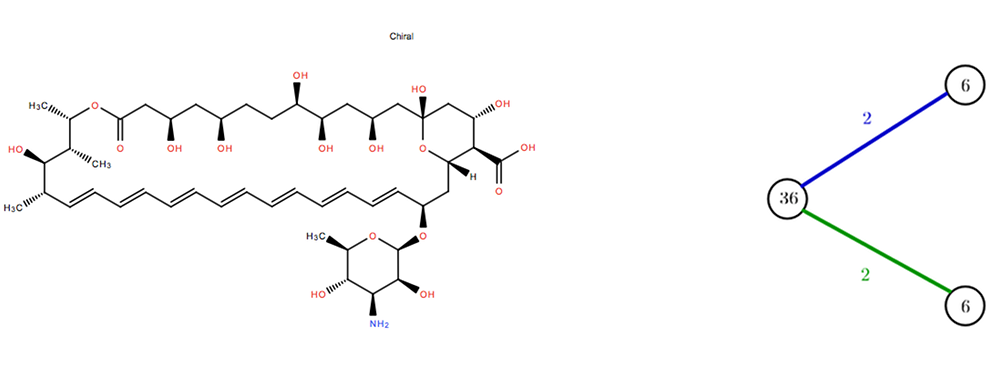
\includegraphics[scale=0.75]{amphotericin3.png}
\end{center}
\caption{Le graphe moleculaire et le graphe de cycles de l'Amphotéricin B.}
\end{figure}

\paragraph{} Dans ce chapitre, nous avons définit formellement le graphe de cycles. Pour le calculer, nous utilisons l'algorithme de McKay pour la numérotation canonique des sommets du graphe moléculaire et ensuite l'algorithme de Horton pour construire un générateur canonique. Par la suite, nous rajoutons éventuellement des cycles supplémentaires pour assurer la canonicité du graphe de cycles. Le choix du paramètre $j$ sera important pour mesurer la similarité dans le chapitre suivant et permet de valider le modèle de graphe de cycles.